\documentclass{beamer}

\mode<presentation> {
\usetheme{Madrid}
}

\beamertemplatenavigationsymbolsempty

% pacman.sty does not allow numbering pages properly with backup/appendix slides
% \usepackage{pacman} % Allows you to be the best presentator ever :D

\usepackage{graphicx} % Allows to include figures
% \usepackage{booktabs} % Allows the use of \toprule, \midrule and \bottomrule in tables
% \usepackage[utf8]{inputenc}
% \usepackage{float}
% \usepackage{mathtools}
% \usepackage{xcolor}
% \usepackage{bm}
% \usepackage{scalerel}
% \usepackage{setspace}
\usepackage{appendixnumberbeamer} % add \appendix

% \usepackage{amsmath}
% \usepackage{amssymb}
\usepackage{mathtools, nccmath}
% \usepackage[mathscr]{euscript}  % euler script font
% \usepackage{cleveref}
% \usepackage{enumitem}

\usepackage{algorithm}
\usepackage[noend]{algpseudocode}

\DeclareMathOperator{\Var}{Var}
\DeclareMathOperator{\modexp}{mod\_exp}
\DeclareMathOperator{\decryptiontime}{decryption\_time}
\DeclareMathOperator{\extrareduction}{extra\ reduction}

%---------------------------------------------------------------------------------------
%	TITLE PAGE
%---------------------------------------------------------------------------------------

\title[DSP - 2021/22 - Lorenzo Palloni]{Timing Attacks against RSA}
\subtitle{(Data Security and Privacy)}
\author{Lorenzo Palloni}
\institute[]{
  University of Florence\\
  \medskip
  \textit{lorenzo.palloni@stud.unifi.it}
}
\date{\today}

\begin{document}

\begin{frame}
\titlepage % Print the title page as the first slide
\end{frame}

%---------------------------------------------------------------------------------------
%	PRESENTATION SLIDES
%---------------------------------------------------------------------------------------
%   TABLE OF CONTENTES
%---------------------------------------------------------------------------------------
%\begin{frame}
%\tableofcontents
%\end{frame}
%---------------------------------------------------------------------------------------
%---------------------------------------------------------------------------------------
\begin{frame}
\frametitle{Introduction}

\begin{itemize}
  \item Main project goal $\rightarrow$ overview of two major timing attacks:
  \begin{itemize}
    \item Kocher's timing attack (1996) \cite{bib:kocher};
    \item Brumley and Boneh's timing attack (2005) \cite{bib:openssl}.
  \end{itemize}
\end{itemize}

\begin{itemize}
  \item A timing attack is a type of side-channel attack.
  \item A side-channel attack exploits physical parameters, such as:
  \begin{itemize}
    \item execution time;
    \item electromagnetic emission;
    \item supply current.
  \end{itemize}
\end{itemize}

\end{frame}
%---------------------------------------------------------------------------------------
\begin{frame}
\frametitle{Square-and-multiply modular exponentiation}

\begin{algorithm}[H]
\caption{Square-and-multiply modular exponentiation algorithm.}\label{alg:one}
\begin{algorithmic}[1]
\Function{$\modexp$}{$y, x, n$}
  \Comment{Computes $y^x \bmod n$}
  \State $R \leftarrow 1$\;
  \For{$k \leftarrow 0, w - 1$}
    \State $R \leftarrow (R \cdot R) \bmod n$\;
    \If{ $\text{(the } $k$ \text{-th bit of } $x$ \text{) is }1$ }
      \State $R \leftarrow (R \cdot y) \bmod n$\;
    \EndIf
  \EndFor
  \State \Return $R$
\EndFunction
\end{algorithmic}
\end{algorithm}

$\modexp$ is a core operation in public-key cryptosystems, such as:
\begin{itemize}
  \item RSA;
  \item Diffie-Hellman key exchange.
\end{itemize}

\end{frame}
%---------------------------------------------------------------------------------------
\begin{frame}
\frametitle{Kocher's timing attack - assumptions}

Assume an RSA cryptosystem, with $D_k[x] = y^x \bmod n$.

Now, suppose that an attacker:

\begin{itemize}
  \item wants to retrieve the private exponent $x$;
  \item already knows the first $b$ exponent bits of $x$;
  \item can perform as many decryption operations as he wants;
  \item is able to measure $T := e + \sum_{i=0}^{k-1} t_i$, where:
  \begin{itemize}
    \item $t_i$ $\rightarrow$ $i$-th iteration required time for $\modexp(y, x, n)$;
    \item $y$ $\rightarrow$ any ciphertext;
    \item $e$ $\rightarrow$ overhead time.
  \end{itemize}
\end{itemize}

\end{frame}
%---------------------------------------------------------------------------------------
\begin{frame}
\frametitle{Kocher's timing attack - pseudocode}

\begin{algorithm}[H]
\caption{Kocher's timing attack}\label{alg:two}
\begin{algorithmic}[1]
  \State generate $s$ ciphertexts $\{ y_1, \dots, y_s \}$;
  \State guess the $b$-th exponent bit $d_b' := 0$;
  \State measure $T'_j = e + \sum_{i = 0}^{b - 1} t'_i, \hspace{1cm} \forall j \in \{ 1, \dots, s\}$;
  \State estimate $\Var(T - T')$;
  \State repeat from step 3. and step 4. with $d'_b := 1$;
  \State choose $d^*_b \in \{0, 1\}$ that minimizes $\Var(T - T')$;
  \State set $d_b \leftarrow d^*_b$;
  \State set $b \leftarrow b + 1$;
  \State repeat from step 2. until $b > k - 1$.
\end{algorithmic}
\end{algorithm}

In step 3., $T'$ is measured by running $\modexp(y, x_b, n)$, where:
\begin{itemize}
  \item $x_b := (d_0 d_1 \cdots d_{b-1} d'_b)_2$.
\end{itemize}

\end{frame}
%---------------------------------------------------------------------------------------
% \begin{frame}
% \frametitle{Kocher's timing attack - why it works}
%
% \begin{itemize}
%   \item
% \end{itemize}
%
% \end{frame}
%---------------------------------------------------------------------------------------
\begin{frame}
\frametitle{Brumley and Boneh's timing attack - assumptions}

Assume an RSA cryptosystem implemented with OpenSSL (0.9.7).

Let $n = pq$ be the public modulus, with $q < p$.

Now, suppose that an attacker:

\begin{itemize}
  \item wants to retrieve the private factor $q$;
  \item knows $i - 1$ bits of $q$: $\{q_0, q_1, \dots, q_{i - 1}\}$;
  \item starts to guess $q$ with $g$:
  \begin{itemize}
    \item[$\rightarrow$] $g_0 := q_0,\ g_1 := q_1,\ \dots,\ g_{i - 1} := q_{i - 1}$;
    \item[$\rightarrow$] $g_i := 0,\ g_{i + 1} := 0,\ \dots,\ g_{k - 1} := 0$;
  \end{itemize}
  \item can perform as many decryption operations as he wants;
  \item knows that his guess $g \in [2^{511}, 2^{512} - 1]$ \footnote{The public modulus $n$ in OpenSSL 0.9.7 has a 1024-bit binary representation.}.

\end{itemize}

\end{frame}
%---------------------------------------------------------------------------------------
\begin{frame}
\frametitle{Brumley and Boneh's timing attack - pseudocode}

\begin{algorithm}[H]
\caption{Brumley and Boneh's timing attack against OpenSSL}\label{alg:three}
\begin{algorithmic}[1]
  \State set $g' := g$, then $g'_i := 1$;
  \State compute $u_g = gR^{-1} \bmod n$, and $u_{g'} = g'R^{-1} \bmod n$;
  \State measure $t_1 = \decryptiontime(u_g)$, and $t_2 = \decryptiontime(u_{g'})$;
  \State compute $\Delta = \left| t_1 - t_2 \right|$;
  \State \Return $0$ if $\Delta$ is "large". Otherwise ($\Delta$ is "small"), \Return $1$.
\end{algorithmic}
\end{algorithm}

Note that in step 1., if $q_i = 1$:
\begin{itemize}
  \item then $g < g' < q$;
  \item otherwise, $g < q < g'$.
\end{itemize}

\end{frame}
%---------------------------------------------------------------------------------------
\begin{frame}
\frametitle{Brumley and Boneh's timing attack - why it works}

Techniques implemented in OpenSSL (0.9.7) to improve $\modexp$:
\begin{itemize}
  \item Chinese Remainder $\rightarrow$ exposes $q$ $\Rightarrow p = n / q \Rightarrow d = e^{-1} \bmod \phi(n)$ \footnote{$\phi(n) = \phi(p) \cdot \phi(q) = (p - 1) \cdot (q - 1).$};
  \item Sliding Windows \cite{bib:sliding} $\rightarrow$ many multiplications by $g$;
  \item Montgomery multiplication \cite{bib:montgomery} $\rightarrow$ more time required when $g < q$ \cite{bib:schindler};
  \item Karatsuba's algorithm $\rightarrow$ less time required when $g$ approaches $q$ from below.
\end{itemize}

\end{frame}
%---------------------------------------------------------------------------------------
\begin{frame}
\frametitle{Brumley and Boneh's timing attack - simulations}

Time variations for each guessed bit ($32$-bits factor):
\begin{itemize}
  \item without blinding (left): almost deterministic;
  \item with blinding (right): unpredictable.
\end{itemize}

\begin{columns}[t]
  \column{.5\textwidth}
    \centering
    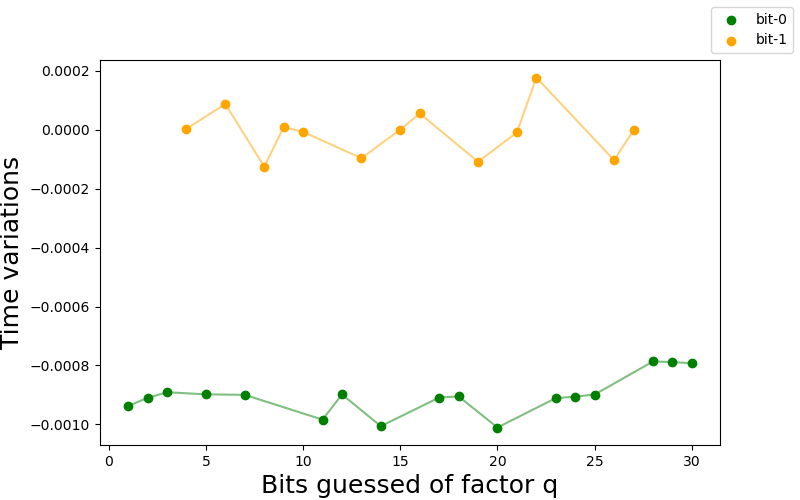
\includegraphics[width=1.0\textwidth]{figures/backup-attack_without_blinding}
  \column{.5\textwidth}
    \centering
    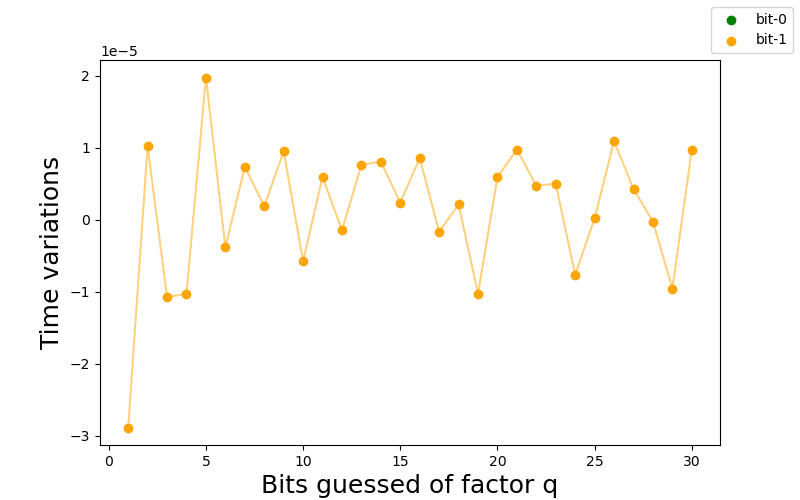
\includegraphics[width=1.0\textwidth]{figures/backup-attack_with_blinding}
\end{columns}

\end{frame}
%---------------------------------------------------------------------------------------
\begin{frame}
\frametitle{Conclusion}

In 1996, Kocher:
\begin{itemize}
  \item showed that simple $\modexp$ exposes the exponent;
  \item prompted improvements on $\modexp$ implementations.
\end{itemize}

In 2005, Brumley and Boneh:
\begin{itemize}
  \item proved that remote timing attacks are practical;
  \item made crypto libraries to implement blinding by default.
\end{itemize}

\end{frame}

%---------------------------------------------------------------------------------------
%---------------------------------------------------------------------------------------
%---------------------------------------------------------------------------------------
%---------------------------------------------------------------------------------------
%---------------------------------------------------------------------------------------
%---------------------------------------------------------------------------------------
\begin{frame}[c,noframenumbering]

  {\Huge \emph{Thanks for your attention!}}

  \begin{itemize}
    \item[]
    \item[]
  \end{itemize}

  \LARGE Do you have any questions?

\end{frame}
%---------------------------------------------------------------------------------------
\begingroup
\footnotesize
\begin{frame}[noframenumbering]
\frametitle{References}
\begin{thebibliography}{99}

\bibitem{bib:kocher}{Kocher, P.C., 1996, August. Timing attacks on implementations of Diffie-Hellman, RSA, DSS, and other systems. In Annual International Cryptology Conference (pp. 104-113). Springer, Berlin, Heidelberg.}
\bibitem{bib:openssl}{Brumley, D. and Boneh, D., 2005. Remote timing attacks are practical. Computer Networks, 48(5), pp.701-716.}
\bibitem{bib:boreale}{Boreale, M., 2003. Note per il corso di Sicurezza delle Reti.}
\bibitem{bib:montgomery}{Montgomery, P.L., 1985. Modular multiplication without trial division. Mathematics of computation, 44(170), pp.519-521.}
\bibitem{bib:sliding}{Menezes, A.J., Van Oorschot, P.C. and Vanstone, S.A., 2018. Handbook of applied cryptography. CRC press.}
\bibitem{bib:schindler}{Schindler, W., 2000, August. A timing attack against RSA with the chinese remainder theorem. In International Workshop on Cryptographic Hardware and Embedded Systems (pp. 109-124). Springer, Berlin, Heidelberg.}
\bibitem{bib:coppersmith}{Coppersmith, D., 1997. Small solutions to polynomial equations, and low exponent RSA vulnerabilities. Journal of cryptology, 10(4), pp.233-260.}

\end{thebibliography}
\end{frame}
\endgroup
%---------------------------------------------------------------------------------------
%---------------------------------------------------------------------------------------
%---------------------------------------------------------------------------------------
%---------------------------------------------------------------------------------------
%---------------------------------------------------------------------------------------
\appendix
%---------------------------------------------------------------------------------------
%---------------------------------------------------------------------------------------
%---------------------------------------------------------------------------------------
%---------------------------------------------------------------------------------------
%---------------------------------------------------------------------------------------
\begin{frame}[c,noframenumbering]

  \Huge Appendix

\end{frame}
%---------------------------------------------------------------------------------------
\begin{frame}
\frametitle{Appendix - Variance estimation in Kocher's attack}

The quantity $\Var(T - T')$ can be estimated with the formula $$\
  \frac{1}{s - 1}\sum_{j = 1}^s \left( \
    (T_j - T'_j) - \frac{1}{s}\sum_{j = 1}^s (T_j - T'_j) \
  \right)^2, \
$$
recalling that:
\begin{itemize}
  \item $s$ is the number of generated ciphertexts;
  \item $T_j$ is the sum of the time required to decrypt the $j$-th ciphertext;
  \item $T'_j = e + \sum_{i = 0}^{b - 1} t'_i, \hspace{1cm} \forall j \in \{ 1, \dots, s\}$;
  \item $e$ is the overhead time required by the attacker custom decryption;
  \item $b - 1$ is the index of the guessed bit.
\end{itemize}

\end{frame}
%---------------------------------------------------------------------------------------
\begin{frame}
\frametitle{Probability of a correct guess in Kocher's attack (1/5)}

An attacker is performing the $b$-th iteration of the Kocher's attack.

We can estimate the probability that $d^*_b$ is correct.

Suppose the attacker:
\begin{itemize}
  \item knows the first $b - 1$ bits of the private exponent $x$;
  \item can measure $T' = \sum_{i = 0}^{b - 1} t'_i$ for each ciphertext $y_j$, with $j \in \{ 1, \dots, s \}$;
\end{itemize}
If $x_b$ is correct, $T - T'$ yields $e + \sum_{i = 0}^{k - 1} t_i - \sum_{i = 0}^{b - 1} t_i = e + \sum_{i = b}^{k - 1} t_i$.

\end{frame}
%---------------------------------------------------------------------------------------
\begin{frame}
\frametitle{Probability of a correct guess in Kocher's attack (2/5)}

Now, assume that:
\begin{itemize}
  \item all the time measurements i.i.d. as $\mathcal{N}(0, 1)$;
  \item $\Var(T_j - T'_j) = \Var(e + \sum_{i = b}^{k - 1} t_i)$ for each ciphertext $y_j$;
  \item the expected variance among all ciphertexts: $\Var(e) + (k - b)\nu$, with $\nu := \Var(t_i)\ \forall i$.
\end{itemize}
However, if only the first $c < b$ bits of the exponent guess are correct, the expected variance will be $\Var(e) + (k + b - 2c)\nu$.

\end{frame}
%---------------------------------------------------------------------------------------
\begin{frame}
\frametitle{Probability of a correct guess in Kocher's attack (3/5)}

Finally, assuming $\Var(e)$ negligible, we can state that the following two probabilities are the same:

\begin{enumerate}
  \item that subtracting a correct $t'_b$ from each ciphertext will reduce the total variance more than subtracting an incorrect $t'_b$;
  \item that $d^*_b$ is correct.
\end{enumerate}

In the next two slides, we will show formulas to attain the first probability.
\end{frame}
%---------------------------------------------------------------------------------------
\begin{frame}
\frametitle{Probability of a correct guess in Kocher's attack (4/5)}

{\scriptsize
\begin{gather*}
Pr \left[
  \frac{1}{s - 1}
  \sum\limits_{j = 1}^{s} \left(
    \sqrt{k - b} X_j  + \sqrt{2(b - c)} Y_j - 0
  \right)^2
  > \frac{1}{s - 1}\sum\limits_{j = 1}^{s} \left(
    \sqrt{k - b} X_j - 0
  \right)^2
\right] \\
= Pr \left[
  (k - b) \sum\limits_{j = 1}^{s} X_j^2
  + 2(b - c) \sum\limits_{j = 1}^{s} Y_j^2
  + \sqrt{2(b - c)(k - b)} \sum\limits_{j = 1}^{s} X_j Y_j
  > (k - b) \sum\limits_{j = 1}^{s} X_j^2
\right] \\
= Pr \left[
  2(b - c) \sum\limits_{j = 1}^{s} Y_j^2
  + \sqrt{2(b - c)}\sqrt{k - b} \sum\limits_{j = 1}^{s} X_j Y_j
  > 0
\right] \\
= Pr \left[
  2 \sqrt{ 2(b - c)(k - b) } \sum\limits_{j = 1}^{s} X_j Y_j
  + 2(b - c) \sum\limits_{j = 1}^{s} Y_j^2 > 0
\right]
\end{gather*}
}
where {\scriptsize $X \sim \mathcal{N}(0, 1)$ } and {\scriptsize $Y \sim \mathcal{N}(0, 1)$ }.
\end{frame}
%---------------------------------------------------------------------------------------
\begin{frame}
\frametitle{Probability of a correct guess in Kocher's attack (5/5)}
Moreover, for $s$ large enough:
{\scriptsize
  \begin{itemize}
    \item $\sum_{j = 1}^{s}Y_j^2 \approx s$
    \item $\sum_{j = 1}^{s}X_jY_j \sim \mathcal{N}(0, \sqrt{s})$,
  \end{itemize}
}
yielding

{\scriptsize
  \begin{align*}
  Pr \left(
    2\sqrt{2(b - c)(k - b)} \left( \sqrt{s} Z \right)
      + 2(b - c)s > 0
  \right) &= Pr \left(
    Z > - \frac{ \sqrt{s(b - c)} }{2(k - b)}
  \right) \\
  &= Pr \left(
    Z < \frac{\sqrt{s(b - c)}}{2(k - b)}
  \right) \\
  &= \Phi \left( \sqrt{ \frac{s(b - c)}{2(k - b)} } \right)
  \end{align*}
}

where {\scriptsize $\Phi(x)$ } is the cumulative density function of {\scriptsize $\mathcal{N}(0, 1)$ }.

\end{frame}
%---------------------------------------------------------------------------------------
%---------------------------------------------------------------------------------------

% To compute the probability that Oscar correctly guesses the $b$-th exponent bit with $x_b$, given that he already knows the real values of the first $b - 1$ bits out of the total amount of $k$ bits, some preliminary assumptions and reasoning are necessary.

% Given $x_b$, Oscar can measure $T' = \sum_{i = 0}^{b - 1} t'_i$ for each ciphertext $y_j$, with $j \in \{ 1, \dots, s \}$.
% If $x_b$ is correct, $T - T'$ yields $e + \sum_{i = 0}^{k - 1} t_i - \sum_{i = 0}^{b - 1} t_i = e + \sum_{i = b}^{k - 1} t_i$.

% Now, it should be reasonable to assume all the time measurements i.i.d. as $\mathcal{N}(0, 1)$. In other words, times $t_i$ and $t'_i$ are all independent and identical distributed as a normal distribution with mean equal to $0$, and standard deviation equal to $1$, called standard normal distribution, and also denoted by $Z$.
%
% Thus, since for each ciphertext $y_j$, we have $\Var(T_j - T'_j) = \Var(e + \sum_{i = b}^{k - 1} t_i)$, the variance among all ciphertexts is expected to be $\Var(e) + (k - b)\nu$, with $\nu := \Var(t_i)\ \forall i$. However, if only the first $c < b$ bits of the exponent guess are correct, the expected variance will be $\Var(e) + (k + b - 2c)\nu$.
%
% Finally, assuming $\Var(e)$ negligible, the probability of a correct guess for Oscar can be computed as the probability that subtracting a correct $t'_b$ from each ciphertext will reduce the total variance more than subtracting an incorrect $t'_b$, and can be obtained with the following steps:
%
% \begin{gather*}
% Pr \left[
%   \frac{1}{s - 1}
%   \sum\limits_{j = 1}^{s} \left(
%     \sqrt{k - b} X_j  + \sqrt{2(b - c)} Y_j - 0
%   \right)^2
%   > \frac{1}{s - 1}\sum\limits_{j = 1}^{s} \left(
%     \sqrt{k - b} X_j - 0
%   \right)^2
% \right] \\
% = Pr \left[
%   (k - b) \sum\limits_{j = 1}^{s} X_j^2
%   + 2(b - c) \sum\limits_{j = 1}^{s} Y_j^2
%   + \sqrt{2(b - c)(k - b)} \sum\limits_{j = 1}^{s} X_j Y_j
%   > (k - b) \sum\limits_{j = 1}^{s} X_j^2
% \right] \\
% = Pr \left[
%   2(b - c) \sum\limits_{j = 1}^{s} Y_j^2
%   + \sqrt{2(b - c)}\sqrt{k - b} \sum\limits_{j = 1}^{s} X_j Y_j
%   > 0
% \right] \\
% = Pr \left[
%   2 \sqrt{ 2(b - c)(k - b) } \sum\limits_{j = 1}^{s} X_j Y_j
%   + 2(b - c) \sum\limits_{j = 1}^{s} Y_j^2 > 0
% \right]
% \end{gather*}
%
% where $X \sim Z$ and $Y \sim Z$. Moreover, for $s$ large enough, $\sum_{j = 1}^{s}Y_j^2 \approx s$, and $\sum_{j = 1}^{s}X_jY_j \sim \mathcal{N}(0, \sqrt{s})$, yielding
%
% \begin{align*}
% Pr \left(
%   2\sqrt{2(b - c)(k - b)} \left( \sqrt{s} Z \right)
%     + 2(b - c)s > 0
% \right) &= Pr \left(
%   Z > - \frac{ \sqrt{s(b - c)} }{2(k - b)}
% \right) \\
% &= Pr \left(
%   Z < \frac{\sqrt{s(b - c)}}{2(k - b)}
% \right) \\
% &= \Phi \left( \sqrt{ \frac{s(b - c)}{2(k - b)} } \right)
% \end{align*}
%
% where $\Phi(x)$ is the cumulative density function (CDF) of $Z$.

%---------------------------------------------------------------------------------------
%---------------------------------------------------------------------------------------
% \begin{frame}
% \frametitle{Experiments - Kocher}
%
% % \begin{itemize}
% %   \item Kocher mainly showed that timing attacks are a real threat for $\modexp$.
% %   \item The attacker only needs 4 times the number of the operations done by the victim.
% % \end{itemize}
%
% % Kocher showed that the theoretical probability of a correct guess (described in \Cref{subsub:guess}) is significantly close to the empirical one computed in the experiment. Specifically, with an expected probability of $\sim 0.84$, among 2450 trials, $~88.5\%$ of them were correct guesses, using a sample size $s = 250$ for each trial.
%
% \end{frame}
%---------------------------------------------------------------------------------------
% \begin{frame}
% \frametitle{Experiments - Brumley and Boneh}
%
% Main takeaways from Brumley and Boneh experiments:
% \begin{enumerate}
%   \item they provided a formula to approximate how many decryptions are required to recover an RSA factor: $$ 2ns \cdot log_2 \left( N/4 \right), $$
%     where:
%     \begin{itemize}
%       \item $n$ is the neighborhood size;
%       \item $s$ is the sample size;
%       \item $N$ is the public RSA modulus.
%     \end{itemize}
% %
% %   \item Second, they used three distinct keys, showing a correlation between keys and the zero-one gap created by the differences $|T_g - T'_g|$ when a bit of $q$ is 0 or 1. As we already mentioned in \Cref{subsec:openssl}, the larger the gap, the greater the chance that $q$ is $0$. Another fact that was pointed out, was that the zero-one gap can be expanded by increasing the neighborhood size, reducing the chance of error, especially when bits hard to guess are encountered.
% %
% %   \item Third, they concluded that users of binary crypto libraries, should be aware of the compile-time options and exact execution environment, to understand the risk of their timing attack. This is due to the fact that slight changes, in combinations of system and compilation settings, can lead to huge changes in zero-one gap estimations.
% %
% %   \item Fourth, they implemented a minor patch for OpenSSL, that was accepted for future incorporation. Their goal was to increase evidence in suggesting that developers should be careful in relying on timing attack tests. Despite their patch decreases the zero-one gap, others can lead to an increment of it.
% %
% %   \item Fifth, they showed that local network timing attacks are practical. They also provided an upper bound of approximately $1$ms for the zero-one gap to judge a network vulnerable.
% %
% %   \item Sixth, they highlighted the difficulty in estimating the minimum number of decryption operations that a successful attack would require. They performed two attacks against two networks that were equal for the majority of the involved parameters except they were distinct in the number of network switches. Surprisingly, the network with less switches (only one) presented in average a zero-one gap that was smaller than the average zero-one gap encountered in the other network. Nevertheless, an important aspect of this experiment is that the attacks worked even in a large network.
%
% \end{enumerate}
%
% \end{frame}
%---------------------------------------------------------------------------------------

\end{document}

